\documentclass[final]{article}

\usepackage{APS360}
\usepackage[utf8]{inputenc} % allow utf-8 input
\usepackage[T1]{fontenc}    % use 8-bit T1 fonts
\usepackage{hyperref}       % hyperlinks
\usepackage{url}            % simple URL typesetting
\usepackage{booktabs}       % professional-quality tables
\usepackage{amsfonts}       % blackboard math symbols
\usepackage{nicefrac}       % compact symbols for 1/2, etc.
\usepackage{microtype}      % microtypography
\usepackage{xcolor}         % colors
\usepackage{graphicx}
\usepackage{tikz}
\usetikzlibrary{positioning,arrows.meta}

% APS360.sty is a NeurIPS style; with [final] its first-page footer calls an
% undefined \@trackname. Blank the footer instead of editing the course file.
\makeatletter
\renewcommand{\@noticestring}{}
\makeatother

% Student number and email live in student_info.tex, which is git-ignored
% because this repository is public.
\IfFileExists{student_info.tex}{\input{student_info.tex}}{\newcommand{\studentinfo}{Student Number: XXXXXXXXXX, (email omitted)}}

\title{Progress Report:\\ Phone-Level Mispronunciation Detection for Korean Learners of English}

\author{%
  Jinwoo Lee \\
  \studentinfo\\
  \url{https://github.com/lee04jinwoo-sys/aps360-mispronunciation}\\
}

\begin{document}

\maketitle

\vspace{-0.5in}

% DRAFT -- every number below comes from a file in results/ (see README "Reproduce").
% Rewrite in your own words before submitting. Check the page limit on Quercus.


\section*{Brief Project Description}
This project builds a model that listens to a learner reading an English sentence and marks each phone as
\emph{correct} or \emph{mispronounced}. The \textbf{input} is a short spectrogram window around one phone, together
with the phone the speaker \emph{should} have said; the \textbf{output} is the probability that this phone was
mispronounced (Figure~\ref{fig:pipeline}). Korean learners tend to make the same substitutions again and again, such
as \texttt{DH}$\rightarrow$\texttt{D} (``the'' read as ``de'') and \texttt{Z}$\rightarrow$\texttt{S}, and they often
cannot hear these errors in their own speech. Most speaking apps only give one score for the whole sentence, which
does not tell the learner which sound to fix.

Deep learning suits this task because the same phone sounds very different across speakers, voices and
microphones, so hand-set acoustic rules generalize poorly. A CNN can learn the relevant time--frequency patterns
directly from the spectrogram, and the corpus provides over 100,000 labelled phones to learn from. I measure
precision, recall and F1 on the mispronounced class on six speakers never seen in training; the CNN counts as a
success if its F1 beats the baseline for every training seed.

\begin{figure}[!h]
  \centering
  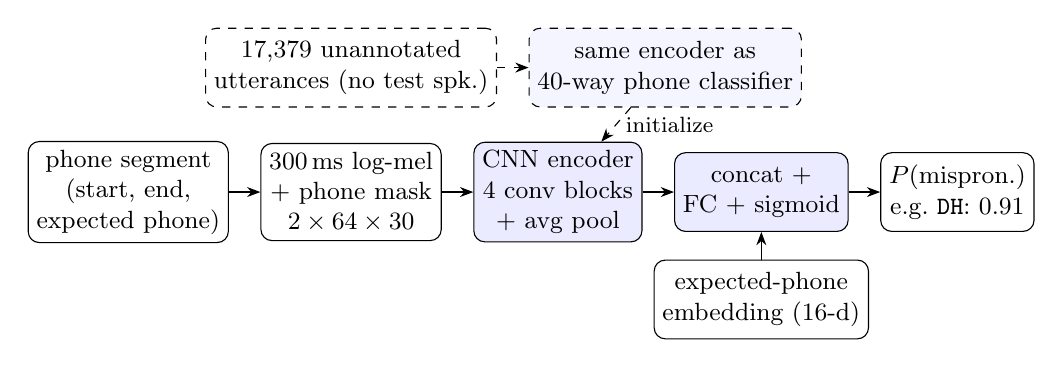
\begin{tikzpicture}[node distance=0.45cm and 0.4cm, every node/.style={font=\small, align=center},
      box/.style={draw, rounded corners, minimum height=1.0cm, inner sep=3pt}, >={Stealth}]
    \node[box] (seg) {phone segment\\ (start, end,\\ expected phone)};
    \node[box, right=of seg] (mel) {300\,ms log-mel\\ + phone mask\\ $2\times64\times30$};
    \node[box, right=of mel, fill=blue!8] (cnn) {CNN encoder\\ 4 conv blocks\\ + avg pool};
    \node[box, right=of cnn, fill=blue!8] (fc) {concat +\\ FC + sigmoid};
    \node[box, right=of fc] (out) {$P$(mispron.)\\ e.g.\ \texttt{DH}: 0.91};
    \node[box, below=0.35cm of fc] (emb) {expected-phone\\ embedding (16-d)};
    \node[box, dashed, above=0.45cm of mel] (unl) {17,379 unannotated\\ utterances (no test spk.)};
    \node[box, dashed, right=of unl, fill=blue!4] (pre) {same encoder as\\ 40-way phone classifier};
    \draw[->] (seg) -- (mel); \draw[->] (mel) -- (cnn); \draw[->] (cnn) -- (fc);
    \draw[->] (emb) -- (fc); \draw[->] (fc) -- (out);
    \draw[->, dashed] (unl) -- (pre);
    \draw[->, dashed] (pre) -- node[right, font=\footnotesize]{initialize} (cnn);
  \end{tikzpicture}
  \caption{Model input and output. The dashed branch is the pre-training stage: the encoder is first trained to
  recognize phones from forced-alignment labels and is then reused for detection.}
  \label{fig:pipeline}
\end{figure}

\section*{Notable Contribution}
\subsection*{Data Processing}
I use L2-ARCTIC v5.0 \cite{zhao2018l2arctic}: 24 speakers from six first languages, 3,599 of whose utterances have
manual phone-level annotations. I read the phone tier of each annotation file and labelled a phone as mispronounced
when the annotator marked it as a substitution or a deletion. Additions were left out, since they have no expected
phone. The audio was resampled to 16\,kHz and turned into a 64-bin log-mel spectrogram (25\,ms window, 10\,ms hop).
Phones are very short (median about 90\,ms), so each sample is a 300\,ms window centred on the phone, plus a second
channel, a binary mask marking the phone's own frames (Figure~\ref{fig:example}). I split the data by speaker so no
voice appears in both training and testing; the test set is the six speakers used in earlier work
\cite{peng2021study} (Table~\ref{tab:split}).

\begin{figure}[!h]
  \centering
  \begin{tikzpicture}[font=\footnotesize]
    \node[inner sep=0] (a) {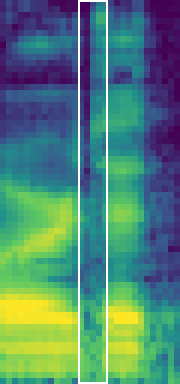
\includegraphics[width=4.6cm,height=2.6cm]{example_1.png}};
    \node[inner sep=0, right=0.8cm of a] (b) {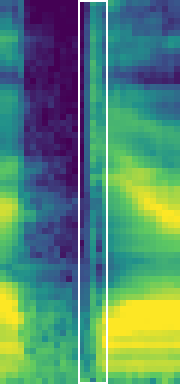
\includegraphics[width=4.6cm,height=2.6cm]{example_2.png}};
    \node[below=1pt of a, align=center] {``\emph{the}'': \texttt{DH} correct (label 0)};
    \node[below=1pt of b, align=center] {``\emph{there}'': \texttt{DH} heard as \texttt{D} (label 1)};
    \node[left=1pt of a, rotate=90, anchor=south] {mel bin $\rightarrow$};
    \node[above=1pt of a] {time (300\,ms) $\rightarrow$};
    \node[above=1pt of b] {time (300\,ms) $\rightarrow$};
  \end{tikzpicture}
  \caption{Two cleaned training samples from Korean speaker HKK (log-mel channel; the white box is the mask, i.e.\
  the phone being judged). The model sees the phone together with its neighbours.}
  \label{fig:example}
\end{figure}

\begin{table}[!h]
\centering
\small
\caption{Speaker-disjoint data split (phones with an expected phone; additions excluded).}
\label{tab:split}
\begin{tabular}{lrrr}
  \toprule
  Split (speakers) & Phones & Mispronounced & Rate \\
  \midrule
  Train (12) & 59,582 & 8,472 & 14.2\% \\
  Validation (6, one per L1) & 29,783 & 4,906 & 16.5\% \\
  Test (6, one per L1) & 29,786 & 4,140 & 13.9\% \\
  \bottomrule
\end{tabular}
\end{table}

\textbf{Challenges.} A deleted phone has no sound of its own, so it was not obvious what its window should contain.
None of the 3,420 deletions has an empty interval: the annotators gave each a short slot (median 40\,ms), and the
mask always marks at least one frame, so every deletion still produces a valid input. A handful of canonical labels
contained typos (e.g.\ \texttt{D\_}) that would have created six extra classes; after cleaning, 40 phones remain.
\textbf{New test data.} Because L2-ARCTIC has only one Korean test speaker, I will record myself reading 50 ARCTIC
prompts and label the phones by listening, starting from a forced alignment, as a never-before-seen test set. If the
labels turn out too unreliable, I will instead test on speechocean762 \cite{zhang2021speechocean}, a separate corpus
with phone-level pronunciation scores.

\subsection*{Baseline Model}
Each phone is summarized by the mean and standard deviation of 13 MFCCs and their first and second derivatives (78
numbers) plus a one-hot expected phone, and classified by a class-weighted logistic regression whose threshold is
chosen on the validation speakers. It reaches a test F1 of 0.431, well above the 0.244 of always predicting
``mispronounced'' (Table~\ref{tab:results}). \textbf{Qualitative result.} On \texttt{DH} and \texttt{TH} the
baseline flags almost every instance (recall 0.998 and 1.00), so its F1 there (0.730, 0.613) equals that of always
guessing ``mispronounced'': for these phones it relies on the phone identity, not the audio. \textbf{Challenge.}
Averaging MFCCs over the phone throws away how the sound changes in time and ignores the neighbouring sounds.

\subsection*{Primary Model}
The CNN has four convolution blocks ($3\times3$ convolution, batch norm, ReLU, $2\times2$ max-pooling; 32, 64, 128
and 128 channels) and global average pooling. The pooled 128-d vector is joined with a 16-d embedding of the expected
phone and passed through a 128-unit hidden layer (dropout 0.3) to a sigmoid output; 260,577 parameters in total. It
is trained with Adam (learning rate $10^{-3}$, batch 256) and binary cross-entropy whose positive class is weighted by
the negative/positive ratio (about 6:1). Training stops when validation F1 has not improved for three epochs, and the
threshold is tuned on the validation speakers. Each run takes about three minutes on a laptop GPU, so I trained five
seeds. In the pre-trained version, the same encoder is first trained as a 40-way phone classifier on 547,208
forced-alignment segments from the 17,379 unannotated utterances of the 18 non-test speakers (76.4\% held-out phone
accuracy), then fine-tuned in exactly the same way.

\begin{table}[!h]
  \centering
  \small
  \caption{Test results, mispronounced class. CNN rows: mean $\pm$ sd over training seeds 0--4.}
  \label{tab:results}
  \begin{tabular}{lccc}
    \toprule
    & Precision & Recall & F1 \\
    \midrule
    Always ``mispronounced'' & 0.139 & 1.000 & 0.244 \\
    Baseline (MFCC + logistic regression) & 0.335 & 0.604 & 0.431 \\
    CNN from scratch & $0.383 \pm 0.031$ & $0.550 \pm 0.042$ & $0.450 \pm 0.013$ \\
    CNN, pre-trained encoder & $0.390 \pm 0.027$ & $0.572 \pm 0.038$ & $\mathbf{0.462 \pm 0.010}$ \\
    \midrule
    Korean speaker YKWK: baseline & 0.362 & 0.635 & 0.461 \\
    Korean speaker YKWK: CNN from scratch & $0.409 \pm 0.032$ & $0.586 \pm 0.046$ & $0.480 \pm 0.019$ \\
    Korean speaker YKWK: CNN, pre-trained & $0.417 \pm 0.046$ & $0.597 \pm 0.067$ & $0.486 \pm 0.009$ \\
    \bottomrule
  \end{tabular}
\end{table}

\begin{figure}[!h]
  \centering
  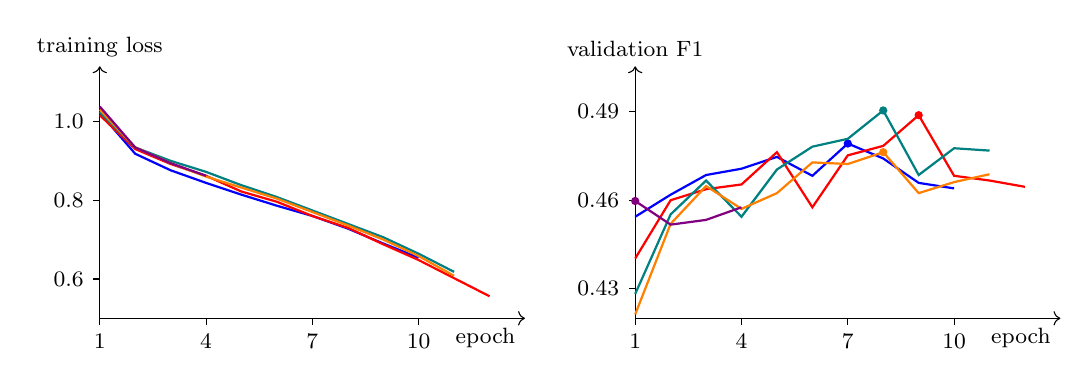
\begin{tikzpicture}[font=\footnotesize]
    % ---- training loss: y = (loss - 0.5) * 5 ----
    \begin{scope}
      \draw[->] (0,0) -- (5.4,0) node[below left]{epoch};
      \draw[->] (0,0) -- (0,3.2) node[above]{training loss};
      \foreach \e in {1,4,7,10} \draw ({0.45*(\e-1)},0) -- ++(0,-0.08) node[below]{\e};
      \foreach \v/\y in {0.6/0.5, 0.8/1.5, 1.0/2.5} \draw (0,\y) -- ++(-0.08,0) node[left]{\v};
\draw[blue, thick] plot coordinates {(0.00,2.61) (0.45,2.09) (0.90,1.88) (1.35,1.72) (1.80,1.57) (2.25,1.43) (2.70,1.30) (3.15,1.14) (3.60,0.95) (4.05,0.77)};
\draw[red, thick] plot coordinates {(0.00,2.58) (0.45,2.15) (0.90,1.96) (1.35,1.81) (1.80,1.61) (2.25,1.48) (2.70,1.30) (3.15,1.15) (3.60,0.94) (4.05,0.74) (4.50,0.51) (4.95,0.28)};
\draw[teal, thick] plot coordinates {(0.00,2.62) (0.45,2.17) (0.90,2.00) (1.35,1.86) (1.80,1.69) (2.25,1.54) (2.70,1.37) (3.15,1.20) (3.60,1.03) (4.05,0.82) (4.50,0.59)};
\draw[orange, thick] plot coordinates {(0.00,2.65) (0.45,2.17) (0.90,1.97) (1.35,1.80) (1.80,1.66) (2.25,1.52) (2.70,1.35) (3.15,1.18) (3.60,1.00) (4.05,0.79) (4.50,0.54)};
\draw[violet, thick] plot coordinates {(0.00,2.69) (0.45,2.17) (0.90,1.97) (1.35,1.81)};
    \end{scope}
    % ---- validation F1: y = (F1 - 0.42) * 37.5 ----
    \begin{scope}[xshift=6.8cm]
      \draw[->] (0,0) -- (5.4,0) node[below left]{epoch};
      \draw[->] (0,0) -- (0,3.2) node[above]{validation F1};
      \foreach \e in {1,4,7,10} \draw ({0.45*(\e-1)},0) -- ++(0,-0.08) node[below]{\e};
      \foreach \v/\y in {0.43/0.375, 0.46/1.5, 0.49/2.625} \draw (0,\y) -- ++(-0.08,0) node[left]{\v};
\draw[blue, thick] plot coordinates {(0.00,1.29) (0.45,1.57) (0.90,1.82) (1.35,1.90) (1.80,2.05) (2.25,1.81) (2.70,2.22) (3.15,2.03) (3.60,1.72) (4.05,1.65)};
\fill[blue] (2.70,2.22) circle (1.5pt);
\draw[red, thick] plot coordinates {(0.00,0.76) (0.45,1.50) (0.90,1.64) (1.35,1.70) (1.80,2.11) (2.25,1.41) (2.70,2.07) (3.15,2.19) (3.60,2.58) (4.05,1.81) (4.50,1.75) (4.95,1.67)};
\fill[red] (3.60,2.58) circle (1.5pt);
\draw[teal, thick] plot coordinates {(0.00,0.31) (0.45,1.32) (0.90,1.75) (1.35,1.29) (1.80,1.89) (2.25,2.18) (2.70,2.28) (3.15,2.64) (3.60,1.82) (4.05,2.16) (4.50,2.13)};
\fill[teal] (3.15,2.64) circle (1.5pt);
\draw[orange, thick] plot coordinates {(0.00,0.05) (0.45,1.20) (0.90,1.68) (1.35,1.39) (1.80,1.59) (2.25,1.98) (2.70,1.96) (3.15,2.11) (3.60,1.59) (4.05,1.73) (4.50,1.83)};
\fill[orange] (3.15,2.11) circle (1.5pt);
\draw[violet, thick] plot coordinates {(0.00,1.49) (0.45,1.19) (0.90,1.25) (1.35,1.41)};
\fill[violet] (0.00,1.49) circle (1.5pt);
    \end{scope}
  \end{tikzpicture}
  \caption{Scratch CNN training curves for the five seeds (one colour per seed; the dot marks the epoch kept by early
  stopping). Training loss keeps going down while validation F1 flattens out around 0.47--0.49, so the model
  starts to overfit after a few epochs.}
  \label{fig:curves}
\end{figure}

\textbf{Quantitative results.} All five scratch seeds beat the baseline, and pre-training raises the mean test F1
from 0.450 to 0.462, with four of five seeds better than the scratch run with the same seed. The gain mostly comes
from precision. The differences are small (about one standard deviation, which covers training seeds only), and the
Korean numbers come from a single speaker. \textbf{Qualitative results.} At its own threshold the scratch CNN flags
more voicing errors than the baseline (48\% vs.\ 26\% of \texttt{D}$\rightarrow$\texttt{T}, 40\% vs.\ 26\% of
\texttt{P}$\rightarrow$\texttt{B}). However, neither CNN uses the audio for \texttt{DH}: its F1 (0.724 scratch, 0.725
pre-trained) stays at the always-``mispronounced'' level, and pre-training even lowers \texttt{TH} (0.569).
\textbf{Challenges.} The model overfits within a few epochs (Figure~\ref{fig:curves}), and the phones that motivate
the project are still not detected from sound.

\section*{Feasibility and Next Steps}
All data processing, the baseline and both CNN variants are done, and one full training run takes minutes, so the
remaining three weeks are enough for: (1)~reducing overfitting with time/frequency masking and stronger dropout;
(2)~testing with forced-alignment instead of hand-marked phone boundaries, which a real tutoring system would not
have; (3)~investigating why \texttt{DH} and \texttt{TH} are not learned, e.g.\ by inspecting their annotations and
training a model on these phones alone; and (4)~collecting and labelling the new Korean test set described above.

\newpage
\bibliographystyle{plain}
\bibliography{references}

\end{document}
